\documentclass[12pt]{article}
\usepackage{graphicx}
\usepackage{hyperref}
\usepackage{cite}

\begin{document}
\title{CSE441 Semester Project: FunCoin}
\author{Rob Kelly\\Sean Turner\\Randy Van Why}
\maketitle

\section{Background}
In October of 2008, a white paper\cite{nakamoto:bitcoin} describing Bitcoin, a decentralized peer-to-peer electronic cash system, was published through cryptography mailing lists. While not the first attempt at an electronic payment-exchange system, Bitcoin was the first entry in the category of digital currencies known as ``cryptocurrencies'', which use concepts from cryptography and cryptographic protocols to secure transaction data. In the Bitcoin system, transactions are cryptographically-signed records of amounts with inputs and outputs -- an input to a transaction is signed to ensure it is only spent by its owner. Transactions are stored as leaves in a Merkle-tree block in the ``blockchain'', a public record of all blocks of all transactions. Bitcoins (also sometimes called ``satoshis'' after the author of the original paper) enter the economy as a reward for ``mining'', which involves finding an arbitrary bitstring nonce that, when combined with the header of the current block in the chain, can be hashed to a value less than some arbitrary difficulty limit. This scheme is called ``proof-of-work'', and is one of several possible block-timestamping solutions. While Bitcoin is the original and most popular cryptocurrency, several alternative cryptocurrencies have been established since, including Litecoin\cite{mcmillan:litecoin}, which uses \textsc{scrypt} instead of \textsc{SHA-256d} as a hashing algorithm, and Peercoin\cite{king:peercoin}, which uses proof-of-stake instead of proof-of-work as a block-timestamping scheme.

Initially, cryptocurrencies were used and promoted solely by cryptography enthusiasts\cite{slashdot:bitcoin} and those with a political interest in a decentralized currency. These early-adopters generally had a clear understanding of the fundamental concepts of cryptography that formed the basis of cryptocurrency protocols, but in more recent years the userbase for cryptocurrencies has expanded to include users who don't have the same background in cryptography. In just a few short years, the use of cryptocurrencies by the general public has grown at an impressive rate, and the effects of this growth are plainly outwardly-visible. The number of new transactions being added to the Bitcoin blockchain has grown from under 10,000 per day prior to 2012 to over 100,000 today, and the Bitcoin mining hash rate has grown from about 20,000 Trillion hashes (GH/s) to over 300,000 GH/s  in 2014 alone. The widespread use of cryptocurrencies has attracted the attention of government agencies\cite{irs:bitcoin}, as well.

\begin{figure}[h!]
  \centering
  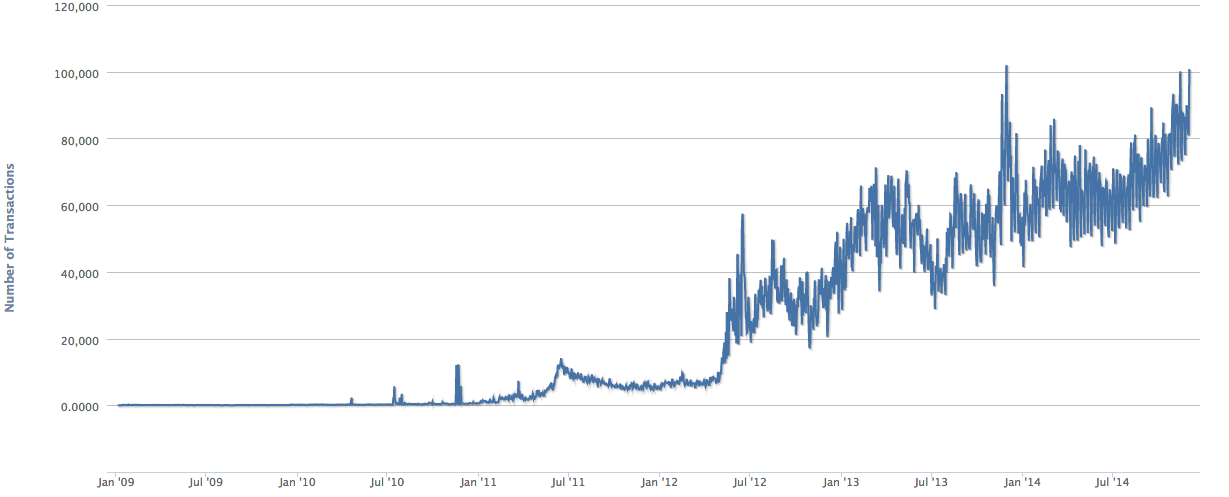
\includegraphics[width=\textwidth]{chart-transactions.png}
  \caption{Number of Bitcoin transactions made per day, 2009-present\cite{blockchain:transactions}}
\end{figure}
\begin{figure}[h!]
  \centering
  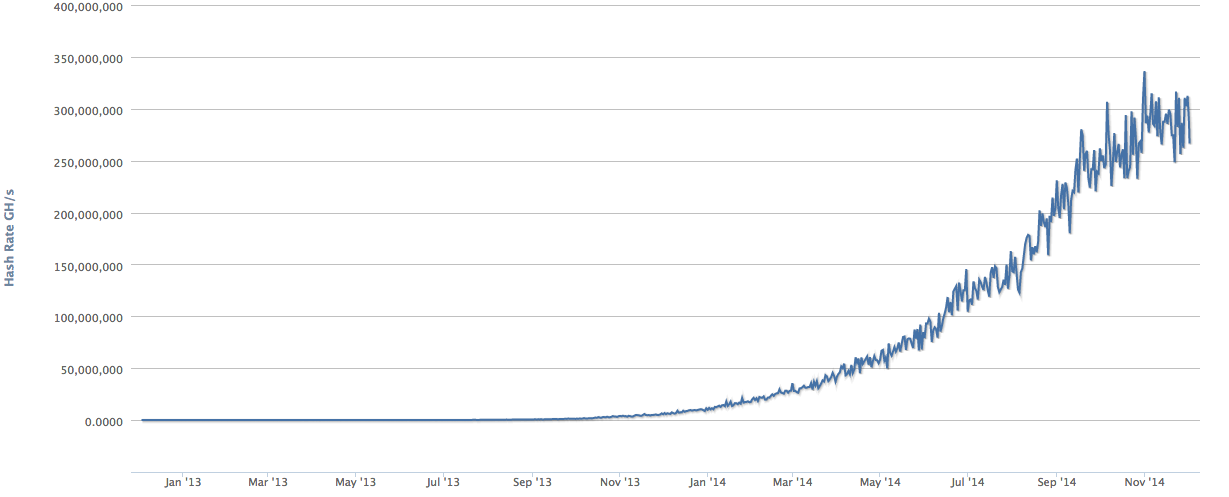
\includegraphics[width=\textwidth]{chart-hashrate.png}
  \caption{Bitcoin mining hash rate in GH/s, 2013-present\cite{blockchain:hashrate}}
\end{figure}

The unprecedented growth of Bitcoin has set off a chain-reaction in public interest in cryptocurrencies, and we expect this trend will only continue as Bitcoin starts to become accepted as a form of payment by more and more vendors\cite{chokun:vendors}. However, the complicated technical nature of the cryptographic foundations of cryptocurrencies as well as the structure and rationale of the protocol itself remain a major stumbling block to public understanding and acceptance of cryptocurrencies. 

\section{OpenSSL}
The group used OpenSSL to handle most of the cryptographic functionality. OpenSSL provides a nice interface for performing digital signitures using DSA.

\section{Approach}
The basic approach we took was to familiarize ourselves with the Bitcoin paper\cite{nakamoto:bitcoin} and the Bitcoin Developer Guide \cite{dev:guide}. 

\subsection{Block Chain}

\section{Discussion}\label{future}
\subsection{Future Work}\label{work}
Some work that can be done to our implementation includes extending it from a simple client/server model to a true peer-to-peer cryptocurrency, making it more modular, so that interested parties may substitute their own implementations of key components such as the block chain and the proof of work in order to gain better understanding of the underlying techniques, and implement true transactions. 

Additional future projects include: implementing a wallet, considering different mining techniques altogether, and following on modularity, possibly making it into a library that can be used to roll your own simplified fun coin.

\subsection{Unsolved Problems}\label{unsolved}
Our biggest unsolved problem (and opportunity for Section \ref{future}) is to decentralize for a more accurate portrayal of how real cryptocurrencies function. Additionally, 

\bibliographystyle{abbrv}
\bibliography{report}

\end{document}
